%@article{madhyastha2015mapping,
%  title={Mapping unseen words to task-trained embedding spaces},
%  author={Madhyastha, Pranava Swaroop and Bansal, Mohit and Gimpel, Kevin and Livescu, Karen},
%  journal={arXiv preprint arXiv:1510.02387},
%  year={2015}
%}

\section{Method Overview} \label{sec:Method}

\begin{figure*}
\centering
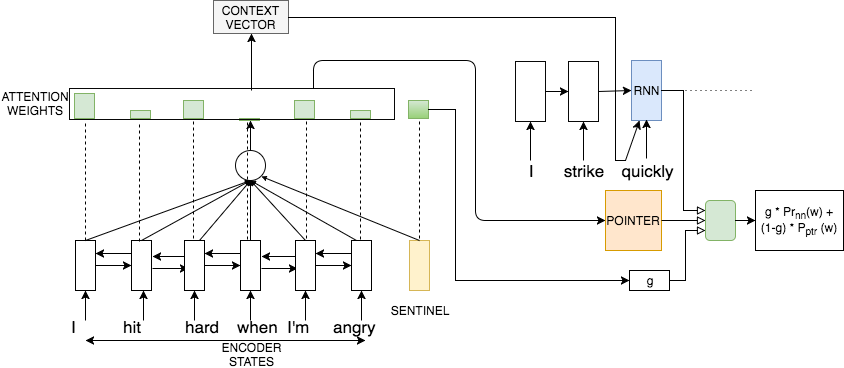
\includegraphics[scale=0.50]{images/StyleTransferGangalVersion.png}
\caption{Pictorial depiction of our overall architecture at decoder step 3. Attention weights are computed using previous decoder hidden state $h_2$, encoder representations, and sentinel vector. Attention weights are shared by decoder RNN and pointer models. The final probability distribution over vocabulary comes from both the decoder RNN and the pointer network. Similar formulation is used over all decoder steps }
\label{fig:architecture}
\end{figure*}


Our overall architecture is shown in Figure (\S\ref{fig:architecture}). We use a bidirectional encoder. We compute soft attention over encoder states. Our decoder side model is a mixture model of RNN module amd pointer network module. The two individual modules share the attentions weights, although it is not necessary to do so. The decoder RNN predicts probability distribution of next word over the vocabulary, while pointer model predicts probability distribution over words in input. The two probabilities undergo a weighted addition, the weights themselves computed based on previous decoder hidden state and the encoder outputs. 

% S2S (sequence-to-sequence) models with attention \cite{bahdanau2014neural} have been used for a variety of tasks like Machine Translation TODO cite. 

Let $\mathbf{x}, \mathbf{y}$ be the some input - output pair in the dataset. Both input $\mathbf{x}$ as well as output $\mathbf{y}$ are sequence of tokens. $\mathbf{x} = \mathbf{x}_1 \mathbf{x}_2 ... \mathbf{x}_{T_{enc}}$, where $T_{enc}$ represents the length of the input sequence $\mathbf{x}$. Similarly, $\mathbf{y} = \mathbf{y}_1 \mathbf{y}_2 ... \mathbf{y}_{T_{dec}} $. Each of $\mathbf{x}_i $, $\mathbf{y}_j $ is be a token from the vocabulary.

\section{Token embeddings} \label{sec:Method2}
Let vocabulary $V$ be the union of modern English and Shakepearean vocabularies i.e. $V = V_{shakespeare} \cup V_{modern}$. Each token is represented by a $M$ dimensional embedding vector. $E_{enc}$ and $E_{dec}$ represent the embedding matrices used by encoder and decoder respectively ( $  E_{enc}, E_{dec} \in \mathbb{R}^{|V| \times M}  $ ). We consider union of the vocabularies for both input and output embeddings because many of the tokens are common in two vocabularies, and in the best performing setting we share embeddings between encoder and decoder models.
Let $E_{enc}(t)$, represent encoder side embeddings of some token $t$. For some input sequence $\mathbf{x}$, $E_{enc}(\mathbf{x})$ is given as $( E_{enc}(\mathbf{x}_1), E_{enc}(\mathbf{x}_2), ... ) $.

\subsection{Pretraining of embeddings}
Considering that we have limited amount of parallel data, learning embeddings in an end-to-end fashion along with the model greatly increases the number of parameters, and is hence not a very good idea.

We pretrain our embeddings on all training sentences. We also experiment with adding additional data from PTB \cite{marcus1993building} for better learning of embeddings. We use the preprocessed PTB data from \cite{mikolov2010recurrent}, which is a standard dataset used in language modelling.

We use the python gensim \footnote{\url{radimrehurek.com/gensim/}} toolkit's implementation of word2vec to train our embeddings. We use four distinct strategies to train our data. In the case where we use external data, we first train the embeddings using both the external data and training data, and then for the same number of iterations on training data alone, to ensure adaptation. Note that we cannot directly use off-the-shelf pre-trained embeddings such as \textit{Glove} \cite{pennington2014glove} and \textit{Word2Vec} \cite{mikolov2013efficient} since we need to learn embeddings for novel word forms (and also different word senses for extant word forms) on the \textit{Original} side.

\subsubsection{Plain}
This method is the simplest pre-training method. Here, we do not use any additional data, and train word embeddings on the union of \textit{Modern} and \textit{Original} sentences. 

\subsubsection{PlainExt}
In this method, we add all the sentences from the external data (\textit{PTB}) to training sentences, and train an embedding on this joint dataset.

\subsubsection{Retro}
\cite{xu2012paraphrasing,xu2014data} also provide a small dictionary $L$ of approximate \textit{Original} $\rightarrow$ \textit{Modern} word pairs, crawled from \url{shakespeare-words.com}, a source distinct from Sparknotes. Since the two \textit{2nd persons} and their corresponding forms (thy, thou, thyself etc) are very frequent but not present in $L$, we add these 4 pairs. Otherwise, we use $L$ as it is. The final dictionary we use has 1524 pairs. \cite{faruqui2014retrofitting} proposed \emph{retrofitting}, a  method to update a learnt set of word embeddings to incorporate pairwise constraints. Given a learnt set of embeddings $p_i \in P$, a vocabulary $V$, and a set $C$ of pairwise constraints $(i,j)$ between words, retrofitting tries to learn a new set of embeddings $q_i \in Q$ to minimize the following objective:
\begin{align*}
    f(Q) & = \delta \sum_{i=1}^{i=|V|} {(p_i-q_i)}^2 + \omega \sum_{(i,j) \in C} {(q_i-q_j)}^2
\end{align*}
We use their off-the-shelf 
implementation \footnote{\url{github.com/mfaruqui/retrofitting}} to encode the dictionary constraints into our pretrained embeddings, setting $C=L$ and using suggested default hyperparameters for $\delta$, $\omega$ and number of iterations.

\subsubsection{RetroExt}
This method is similar to \emph{Retro}, except that we use sentences from the external data (\textit{PTB}) in addition to training sentences.

\subsubsection{None}
Indicates no pretraining.
%\subsubsection{METRO}
%\subsubsection{METROEXT}


%Also, we are hampered by the lack of a standard monolingual dataset for Shakespearean English.

\subsection{\emph{Fixed} embeddings}
Fine-tuning pre-trained embeddings for a given task may lead to \emph{overfitting}, especially in case of small amount of supervised data for the task \cite{madhyastha2015mapping}. This is because embeddings for only a fraction of vocabulary items get updated,  while it doesnt get updated for many vocabulary items. To avoid this, we consider fixed embeddings pretrained as per procedures described earlier. While reporting  results  in Section (\S \ref{sec:Results}), we separately report results for fixed (\emph{FIXED}) and trainable (\emph{VAR}) embeddings, and show that keeping embeddings fixed leads to better performance. 

\section{Method Description} \label{sec:Method3}
In this section we give details of the various modules in the proposed neural model. 

\subsection{Encoder model}
 Let $\overrightarrow{LSTM_{enc}}$ and $\overleftarrow{LSTM_{enc}}$ represent the forward and reverse encoder. $\mathbf{h}^{\overrightarrow{enc}}_{t}$ represent hidden state of encoder model at step $t$ ($\mathbf{h}^{\overrightarrow{enc}}_{t} \in \mathbb{R}^{H} $).
% , the input sequence $\bm{x}$ is of length $I$ and the output sequence $\bm{y}$ is of length $|O|$.
The following equations describe the model:
\begin{center}
\footnotesize
\begin{align*}
    \mathbf{h}^{\overrightarrow{enc}}_0 &=\overrightarrow{0},  \mathbf{h}^{\overleftarrow{enc}}_{|x|} = \overrightarrow{0} \\
    \mathbf{h}^{\overrightarrow{enc}}_{t} &= \overrightarrow{LSTM_{enc}}(\mathbf{h}^{enc}_{t-1},{E_{enc}}({\mathbf{x}_{t}})) \\
    \mathbf{h}^{\overleftarrow{enc}}_{t} &= \overleftarrow{LSTM_{enc}}(\mathbf{h}^{enc}_{t+1},{E_{enc}}({x_{t}})) \\
    \mathbf{h}^{enc}_{t} &= \mathbf{h}^{\overrightarrow{enc}}_{t} + \mathbf{h}^{\overleftarrow{enc}}_{t} 
\end{align*}
\normalsize
\end{center}
We use addition to combine the forward and backward encoder states, rather than concatenation which is standardly used, since it doesn't add extra parameters, which is important in a low-data scenario such as ours. 

%\subsection{Decoder RNN}

\subsection{Attention}

Let $\mathbf{h}_t^{dec}$ represent the hidden state of the decoder LSTM at step $t$. Let $E_{dec}(\mathbf{y}_{t-1})$ represent the decoder side embeddings of previous step output. We use special $START$ symbol at $t=1$. 

We first compute a query vector, which is a linear tranformation of $\mathbf{h}_{t-1}^{dec}$. A sentinel vector $\mathbf{s} \in \mathbb{R}^H$ is concatenated with the encoder states to create $F_{att} \in \mathbb{R} ^ { (T_{enc}+1) \times H } $, where $T_{enc}$ represents the number of tokens in encoder input sequence $\mathbf{x}$. A normalized attention weight vector is computed. The value $g$, which corresponds to attention weight over sentinel vector, represents the weight given to the decoder RNN module while computing output probabilties.
\begin{center}
\footnotesize
\begin{align*}
  \mathbf{q} &= \mathbf{h}_{t-1}^{dec} \,W_{q}   &&  W_{q} \in \mathbb{R}^{H \times H} \\
  F_{att} &= concat( \mathbf{h}^{enc}_{1..T_{enc}}, \mathbf{s} )   && F_{att} \in \mathbb{R}^{(T_{enc}+1) \times H} \\
  \boldsymbol{\alpha}_i &= \sum_{j=1}^{H}( tanh(F_{att}^{(ij)} \, \mathbf{q}_j) ) + \mathbf{b}_i   && \boldsymbol{\alpha}_i, \mathbf{b}_i \in \mathbb{R} \\
  \boldsymbol{\alpha}^{norm} &= softmax(\boldsymbol{\alpha}) && \boldsymbol{\alpha}^{norm} \in \mathbb{R}^{T_{enc}+1} \\
  \boldsymbol{\beta} &= \boldsymbol{\alpha}^{norm}_{1,2,...,T_{enc}} && \boldsymbol{\beta} \in \mathbb{R}^{T_{enc}} \\
  g &= \boldsymbol{\alpha}^{norm}_{T_{enc}+1} && g \in \mathbb{R}
\end{align*}
\normalsize
\end{center}

%  F \,&= \,\text{relu}\, ( I_{proj} \,\oplus\, \mathbf{d}_{proj} ) && F \in \mathbb{R}^{(L+1) \times Q}


\subsection{Pointer model}

%Pointer network
%- motivation: how copy is needed for our task
As noted in (\S \ref{sec:Dataset}), \textit{Original} and \textit{Modern} have significant vocabulary overlap. Moreover, there are lot of proper nouns and rare words which might not be predicted by a sequence to sequence model. To rectify this, pointer networks have been used to enable copying of tokens from input directly \cite{merity2016pointer}. The pointer module provides location based attention, and output probability distribution due to pointer network module can be expressed as follows:
\begin{center}
\footnotesize
\begin{align*}
P_{t}^{PTR}(w) &= \sum_{\mathbf{x}_j=w}( \boldsymbol{\beta}_j )
\end{align*}
\normalsize
\end{center}

\subsection{Decoder RNN}

Output probabilities over vocabulary as per the decoder LSTM module are computed as follows:

% &&  \mathbf{c}_t \in \mathbb{R}^{(L+1) \times Q}
\begin{center}
\footnotesize
\begin{align*}
\mathbf{c}_t &= \sum_{i=1}^{T_{enc}} \boldsymbol{\beta}_i \, \mathbf{h}^{enc}_i  \\
\mathbf{h}^{dec}_{t} &= LSTM(\mathbf{h}^{dec}_{t-1},[\text{concat}({E_{dec}}({\mathbf{y}_{t-1}}),\mathbf{c}_{t})])  \\
P_{t}^{LSTM} &=\text{softmax}(W_{out}[\text{concat}(\mathbf{h}^{dec}_{t}, \mathbf{c}_{t})] + \mathbf{b}^{out}) 
\end{align*}
\normalsize
\end{center}
During training, we feed the ground truth for $\mathbf{y}_{t-1}$, whereas while making predictions on test data, predicted output from previous step is used instead.

\subsection{Output prediction}
As mentioned earlier, final output is a mixture of weighted probabilities from decoder LSTM model and pointer model.  Specifically, output probability of a token $w$ at step $t$ is given as follows:
\begin{center}
\footnotesize
\begin{align*}
P_{t}(w) &= g \times P_{t}^{LSTM}(w) + (1-g) \times P_{t}^{PTR}(w) 
\end{align*}
\normalsize
\end{center}
$P_{t}^{PTR}(w)$ takes a non-zero value only if $w$ occurs in input sequence, otherwise it is $0$.

Setting $g=0$ corresponds to not having a \textit{Copy} component, reducing the model to a plain attentional S2S model, which we refer to as a \textit{SimpleS2S} model. 
%
%
%How are we saving parameters? (expand later)
%\begin{itemize}
%    \item Encoder-decoder embedding sharing
%    \item Pointer-Generation (attention weight) sharing
%    \item Freezing the embeddings 
%\end{itemize}
%
%How are we making learning easier (good starting point)
%\begin{itemize}
%    \item Pretraining embeddings
%    \item Incorporating external dictionary constraints by retrofitting
%    \item Pretraining embeddings on additional monolingual data
%    \item Simple loss function (no auxiliary terms like sentinel loss)
%\end{itemize}
%


\section{Loss functions} \label{sec:Method4}
%Let $i^{th}$ point in dataset be represented by $(\mathbf{x}^{(i)}, \mathbf{y}^{(i)} )$. Let the prediction by model be $\mathbf{y}$

Cross entropy loss is used to train the model.
For a data point $( \mathbf{x}, \mathbf{y} ) \in \mathcal{D}$ and predicted probability distributions $P_t\,(w)$ over the different words $w \in \mathbf{V}$ for each time step $t \in \{1,\ldots,T_{dec}\}$, the loss is given by
\begin{center}
\small
\begin{align*}
  - \sum_{t=1}^{T_{dec}} \,\log p\,\bigl(P_t\,(\mathbf{y}_t) \bigr)
\end{align*}
\normalsize
\end{center}

\subsection{Sentinel Loss (\textsc{SL})}
Following from work by \cite{merity2016pointer}, we consider additional sentinel loss. This loss function can be considered as a form of \emph{supervised attention}. Sentinel loss is given as follows:
\begin{center}
\small
\begin{align*}
  - \sum_{t=1}^{T_{dec}} \,\log ( g^{(t)} + \sum_{x_j=y_t}( \beta^{(t)}_j ) )
\normalsize
\end{align*}
\end{center}


We report the results demonstrating the impact of including the sentinel loss function (\textsc{+SL}).


%\subsection{Initial state of LSTM}
%
%The initial hidden state $h_0$ and initial memory cell state $c_0$ of the LSTM are derived from a transformed combination of the abstract image features produced by the convolutional network, and the input demand embedding.
%For this, we use late fusion on projections of the abstract image features and the demand embedding. The choice of late fusion was driven by the fact that the dimensionality \,($L \times Q$) \,of the image features is much larger than that of the demand embedding. Thus, early fusion may results in the domination of the demand features by the image features.
%
%Let $E_D$ represent embeddings of demand word $D$, and $H$ be the hidden state size of the LSTM network.
%Mathematically, given image features $I_{feats}^{(1)}, \ldots, I_{feats}^{(L)} $ of image $I$, and demand $D$,
%\begin{align}
%  \mathbf{i}_{init} \,&= \,\frac{1}{L} \,\sum_{j=1}^L \Bigl( I_{feats}^{(j)} W_{ih} \Bigr) + \mathbf{b}_{ih} && W_{ih} \in \mathbb{R}^{Q \times (H-M)} \,~\,\text{and} \,~\,\mathbf{b}_{ih} \in \mathbb{R}^{H-M} \\[0.2em]
%  \mathbf{d}_{init} \,&= \,E_d \,W_{dh} + \mathbf{b}_{dh} && W_{dh} \in \mathbb{R}^{M \times M} \,~\,\text{and} \,~\,\mathbf{b}_{dh} \in \mathbb{R}^{M} \\[0.5em]
%  \mathbf{h}_0 \,&= \,\text{tanh}\,(\mathbf{i}_{init}) \,\oplus \,\text{tanh}\,(\mathbf{d}_{init})
%\end{align}